\section{Aspects Reproduced}
\begin{frame}{Indexing and LM}
    \begin{columns}
        \begin{column}{0.5\textwidth}
            \begin{itemize}
                \item Lucene... What version?
            \end{itemize}
            \bigskip
            \begin{itemize}
                \item Indexing... How?
                      \begin{itemize}
                          \item Tokenization
                          \item Stopwords removal
                          \item Transposed index
                      \end{itemize}
            \end{itemize}
            \bigskip
            \begin{itemize}
                \item Base Language Model
            \end{itemize}
        \end{column}
        \begin{column}{0.5\textwidth}

            \bigskip
            
\includegraphics[width=\columnwidth]{img/lucene_logo.png}
            
            \bigskip
            \bigskip
            \bigskip
            \bigskip
            \bigskip
            \bigskip
            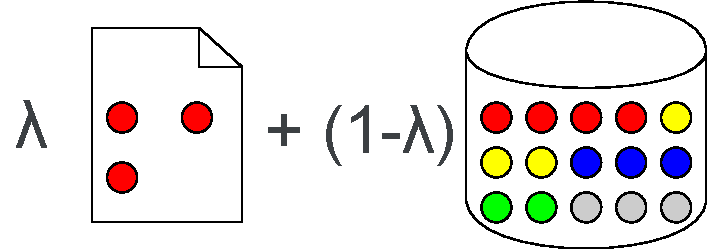
\includegraphics[width=\columnwidth]{img/lm.pdf}
        \end{column}
    \end{columns}
\end{frame}

\begin{frame}{GLM}
    \begin{center}
        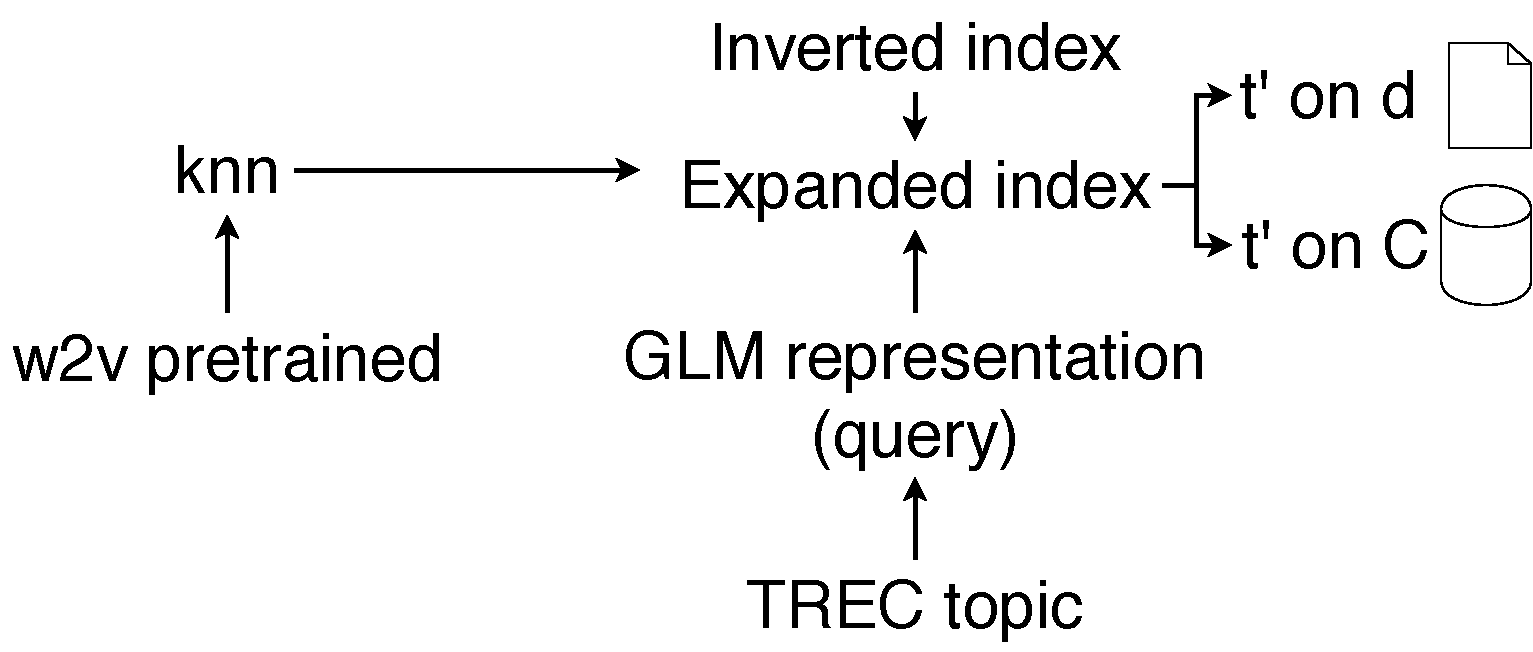
\includegraphics[width=0.8\textwidth]{img/reproduction.pdf}
    \end{center}
    \begin{columns}
        \begin{column}{0.33\textwidth}
            \begin{itemize}
                \item First approach: let's do it ourselves (fail)
            \end{itemize}
        \end{column}
        \begin{column}{0.33\textwidth}
            \begin{itemize}
                \item Second approach: let's try to take example and make it better
            \end{itemize}
        \end{column}
        \begin{column}{0.33\textwidth}
            \begin{itemize}
                \item Is it enough? Time constraints...
            \end{itemize}
        \end{column}
    \end{columns}
\end{frame}
